\documentclass{hw}
\hwname{6 / Radicals / q-1}

\begin{document}

\section*{Quiz 1}
\subsubsection*{1. Simplify}
\begin{enumerate}[label=\alph*.]
    \item $\sqrt{32} \cdot \sqrt{2}$
    \studentlargeworkspace
    \item $-\sqrt{\frac{1}{288}}$
    \studentlargeworkspace
    \item $4x\sqrt{7} \cdot 2\sqrt{14}$
    \studentlargeworkspace
    \item $\sqrt[3]{\frac{8m^3}{27}}$
    \studentlargeworkspace
    \item $\sqrt{162p^2}$
    \studentlargeworkspace
\end{enumerate}

\subsubsection*{2. Complete this table of numbers and their positive square roots}
\begin{center}
    \renewcommand{\arraystretch}{2}
    \begin{minipage}{0.4\textwidth}
    \centering
    \begin{tabular}{|c|c|}
    \hline
    Number & Square Root \\
    \hline
    81 & \blankline{2em} \\
    \blankline{2em} & 12 \\
    9 & \blankline{2em} \\
    256 & \blankline{2em} \\
    \blankline{2em} & 25 \\
    \hline
    \end{tabular}
    \end{minipage}
    \begin{minipage}{0.4\textwidth}
    \centering
    \begin{tabular}{|c|c|}
    \hline
    Number & Square Root \\
    \hline
    169 & \blankline{2em} \\
    484 & \blankline{2em} \\
    \blankline{2em} & 20 \\
    \blankline{2em} & 15 \\
    49 & \blankline{2em} \\
    \hline
    \end{tabular}
    \end{minipage}
\end{center}    

\newpage
\uline{\textit{Extra Credit}}
\subsubsection*{\normalsize Sound Intensity}
\begin{figure}[h]
    \centering
    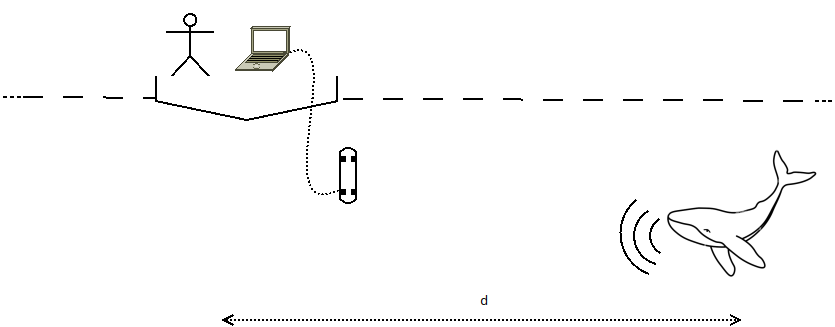
\includegraphics[width=0.9\textwidth]{dia/radicals-whale.png}
    \caption{A whale, whose call is detected by the hydrophone.}
    \label{fig:whale}
\end{figure}

Marine biologists are tracking whales using a hydrophone (underwater microphone) in the ocean.
An average whale’s call has a power of $900 \: watts$.
One morning, the hydrophone detects a whale call with a sound intensity of $0.0001 \: watts/meter^2$. \\
\\
%In this "simplified" universe, the sound intensity follows the equation:
It is known that the sound intensity follows the equation:

{\centering
$I = \frac{P}{d^2}$
\par}

where,
\begin{itemize}
    \item $P$ is the power of the source in $watts$
    \item $I$ is the intensity measured by the receiver in $watts/meter^2$
    \item $d$ is the distance in $meters$
\end{itemize}
\bigskip
What is the distance between the whale and the hydrophone?

% \subsubsection*{\normalsize Solution}
% \begin{align*}
% 0.0001 &= \frac{900}{d^2} \\
% d^2 &= \frac{900}{0.0001} \\
% d^2 &= 9000000 \\
% d &= \sqrt{9000000} \\
% d &= 3000
% \end{align*}
% The distance between the whale and the hydrophone is 3000 meters, or 3 kilometers.

\end{document}